\begin{frame}{General ML selection}
    \begin{columns}
      \begin{column}{0.5\textwidth}
        \centering 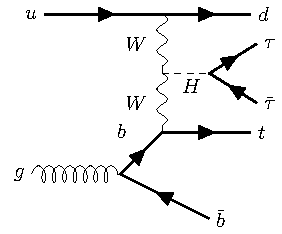
\includegraphics[width=0.8\textwidth]{/cephfs/user/s6chkirf/feynman_diagrams/tHq_tautau}\\
                \begin{itemize}
          \item n-jets: 2 (b-jets: \textbf{1})
          \item b-jet WP: 70 DL1r
          \item nLeptons \& nTaus: $\bf{2e / \mu~1\tau_{\text{had}}} $
          \item $E_{\text{T,miss}}$: no cut (to \SI{800}{GeV})
        \end{itemize}
      \end{column}
      \begin{column}{0.7\textwidth}
        \vspace*{-0.05\textwidth}
        \begin{itemize}
          \footnotesize
          \item jets:
          \vspace*{-0.02\textwidth}
          \begin{itemize}
            \footnotesize
            \item $p_T>\SI{35}{GeV}$
            \item $|\eta|<4.5$
            \item EMPFlow
          \end{itemize}
          \item electrons:
          \vspace*{-0.02\textwidth}
          \begin{itemize}
            \footnotesize
            \item $p_T>\SI{20}{GeV}$ leading \SI{27}{GeV}
            \item $|\eta|<2.5$ not in 1.37 - 1.52
            \item WP: LooseAndBLayerLH ; \\isolation: no requirement
          \end{itemize}
          \item muons:
          \vspace*{-0.02\textwidth}
          \begin{itemize}
            \footnotesize
            \item $p_T>\SI{20}{GeV}$ leading \SI{27}{GeV}
            \item $0.01<|\eta|<2.5$
            \item WP: Loose ; isolation: no requirement
          \end{itemize}
          \item taus:
          \vspace*{-0.02\textwidth}
          \begin{itemize}
            \footnotesize
            \item $p_T>\SI{20}{GeV}$ leading \SI{27}{GeV}
            \item $|\eta|<2.5$ not in 1.37 - 1.52
            \item WP: RNNLoose
            \item ASG recommended OLR ($\tau_{had}$ remove jets)
          \end{itemize}
        \end{itemize}
      \end{column}
    \end{columns}
  \end{frame}


\begin{frame}{Features and weight setup}
  \begin{itemize}
    \item Absolute weights for training because \rightarrow best and most stable results
    \item Preliminary selection of variables
  \end{itemize}
    \begin{columns}
        \begin{column}{0.5\textwidth}
            \resizebox{\linewidth}{!}{
            \begin{tabular}{|l|l|}
                \hline
                eta\_jf          & forward jet eta                        \\ \hline
                pt\_jf           & forward jet transverse momentum        \\ \hline
                mass\_jf         & forward jet mass                       \\ \hline
                phi\_jf          & forward jet phi                        \\ \hline
                eta\_b           & b-jet eta                              \\ \hline
                pt\_b            & b-jet transverse momentum              \\ \hline
                phi\_b           & b-jet phi                              \\ \hline
                HvisMass         & mass of LorentzV sum of hadronic taus  \\ \hline
                m\_met           & Missing energy                         \\ \hline
                Reco\_w\_mass\_2 & Reconstructed mass of the W case 1     \\ \hline
                Reco\_w\_mass\_1 & Reconstructed mass of the W case 2     \\ \hline
            \end{tabular}}
        \end{column}
        \begin{column}{0.5\textwidth}
            \resizebox{\linewidth}{!}{
            \begin{tabular}{|l|l|}
                 \hline
                 deltaRTau        & Delta R of the hadronic taus          \\ \hline
                 deltaPhiTau      & Delta phi of the hadronic taus        \\ \hline
                 HvisPt           & pt of LorentzV sum of hadronic taus      \\ \hline
                 HvisEta          & eta of LorentzV sum of hadronic taus      \\ \hline
                 TvisMass         & mass of reconstructed top             \\ \hline
                 TvisPt           & pt of visible top                     \\ \hline
                 TvisEta          & eta of visible top                    \\ \hline
                 M\_b\_jf         & Mass of LorentV sum of b and jf       \\ \hline
                 HT               & Sum of transverse energies            \\ \hline
                 lep\_Top\_pt     & Light lepton pt                       \\ \hline
                 lep\_Top\_eta    & Light lepton eta                      \\ \hline
             \end{tabular}}
        \end{column}
    \end{columns}
\end{frame}
  


\begin{frame}{Hyperparameters}
  \begin{itemize}
    \item Optimised by small grid search
    \item More thorough optimisation using evolutionary method scheduled, method is in place
  \end{itemize}
    \begin{table}[]
    \begin{tabular}{|l|l|}
    \hline
    Hyperparameter          &     Setting              \\ \hline
    Model                   &     Categorical          \\ \hline
    Nodes                   &     120                  \\ \hline
    Layers                  &     6                    \\ \hline
    Dropout                 &     0.65                 \\ \hline
    Batchnormalisation      &     On                   \\ \hline
    Activation              &     elu                  \\ \hline
    Output activation       &     sigmoid              \\ \hline
    Batch size              &     1000                 \\ \hline
    Optimisation            &     Adam                 \\ \hline
    Weight Initialisation   &     Lecun Normalisation  \\ \hline
    K-folds                 &     4                    \\ \hline
    \end{tabular}
    \end{table}
\end{frame}
  

